% Options for packages loaded elsewhere
\PassOptionsToPackage{unicode}{hyperref}
\PassOptionsToPackage{hyphens}{url}
%
\documentclass[
]{article}
\usepackage{lmodern}
\usepackage{amsmath}
\usepackage{ifxetex,ifluatex}
\ifnum 0\ifxetex 1\fi\ifluatex 1\fi=0 % if pdftex
  \usepackage[T1]{fontenc}
  \usepackage[utf8]{inputenc}
  \usepackage{textcomp} % provide euro and other symbols
  \usepackage{amssymb}
\else % if luatex or xetex
  \usepackage{unicode-math}
  \defaultfontfeatures{Scale=MatchLowercase}
  \defaultfontfeatures[\rmfamily]{Ligatures=TeX,Scale=1}
\fi
% Use upquote if available, for straight quotes in verbatim environments
\IfFileExists{upquote.sty}{\usepackage{upquote}}{}
\IfFileExists{microtype.sty}{% use microtype if available
  \usepackage[]{microtype}
  \UseMicrotypeSet[protrusion]{basicmath} % disable protrusion for tt fonts
}{}
\makeatletter
\@ifundefined{KOMAClassName}{% if non-KOMA class
  \IfFileExists{parskip.sty}{%
    \usepackage{parskip}
  }{% else
    \setlength{\parindent}{0pt}
    \setlength{\parskip}{6pt plus 2pt minus 1pt}}
}{% if KOMA class
  \KOMAoptions{parskip=half}}
\makeatother
\usepackage{xcolor}
\IfFileExists{xurl.sty}{\usepackage{xurl}}{} % add URL line breaks if available
\IfFileExists{bookmark.sty}{\usepackage{bookmark}}{\usepackage{hyperref}}
\hypersetup{
  pdftitle={Basic Regression},
  pdfauthor={Corina Geier},
  hidelinks,
  pdfcreator={LaTeX via pandoc}}
\urlstyle{same} % disable monospaced font for URLs
\usepackage[margin=1in]{geometry}
\usepackage{color}
\usepackage{fancyvrb}
\newcommand{\VerbBar}{|}
\newcommand{\VERB}{\Verb[commandchars=\\\{\}]}
\DefineVerbatimEnvironment{Highlighting}{Verbatim}{commandchars=\\\{\}}
% Add ',fontsize=\small' for more characters per line
\usepackage{framed}
\definecolor{shadecolor}{RGB}{248,248,248}
\newenvironment{Shaded}{\begin{snugshade}}{\end{snugshade}}
\newcommand{\AlertTok}[1]{\textcolor[rgb]{0.94,0.16,0.16}{#1}}
\newcommand{\AnnotationTok}[1]{\textcolor[rgb]{0.56,0.35,0.01}{\textbf{\textit{#1}}}}
\newcommand{\AttributeTok}[1]{\textcolor[rgb]{0.77,0.63,0.00}{#1}}
\newcommand{\BaseNTok}[1]{\textcolor[rgb]{0.00,0.00,0.81}{#1}}
\newcommand{\BuiltInTok}[1]{#1}
\newcommand{\CharTok}[1]{\textcolor[rgb]{0.31,0.60,0.02}{#1}}
\newcommand{\CommentTok}[1]{\textcolor[rgb]{0.56,0.35,0.01}{\textit{#1}}}
\newcommand{\CommentVarTok}[1]{\textcolor[rgb]{0.56,0.35,0.01}{\textbf{\textit{#1}}}}
\newcommand{\ConstantTok}[1]{\textcolor[rgb]{0.00,0.00,0.00}{#1}}
\newcommand{\ControlFlowTok}[1]{\textcolor[rgb]{0.13,0.29,0.53}{\textbf{#1}}}
\newcommand{\DataTypeTok}[1]{\textcolor[rgb]{0.13,0.29,0.53}{#1}}
\newcommand{\DecValTok}[1]{\textcolor[rgb]{0.00,0.00,0.81}{#1}}
\newcommand{\DocumentationTok}[1]{\textcolor[rgb]{0.56,0.35,0.01}{\textbf{\textit{#1}}}}
\newcommand{\ErrorTok}[1]{\textcolor[rgb]{0.64,0.00,0.00}{\textbf{#1}}}
\newcommand{\ExtensionTok}[1]{#1}
\newcommand{\FloatTok}[1]{\textcolor[rgb]{0.00,0.00,0.81}{#1}}
\newcommand{\FunctionTok}[1]{\textcolor[rgb]{0.00,0.00,0.00}{#1}}
\newcommand{\ImportTok}[1]{#1}
\newcommand{\InformationTok}[1]{\textcolor[rgb]{0.56,0.35,0.01}{\textbf{\textit{#1}}}}
\newcommand{\KeywordTok}[1]{\textcolor[rgb]{0.13,0.29,0.53}{\textbf{#1}}}
\newcommand{\NormalTok}[1]{#1}
\newcommand{\OperatorTok}[1]{\textcolor[rgb]{0.81,0.36,0.00}{\textbf{#1}}}
\newcommand{\OtherTok}[1]{\textcolor[rgb]{0.56,0.35,0.01}{#1}}
\newcommand{\PreprocessorTok}[1]{\textcolor[rgb]{0.56,0.35,0.01}{\textit{#1}}}
\newcommand{\RegionMarkerTok}[1]{#1}
\newcommand{\SpecialCharTok}[1]{\textcolor[rgb]{0.00,0.00,0.00}{#1}}
\newcommand{\SpecialStringTok}[1]{\textcolor[rgb]{0.31,0.60,0.02}{#1}}
\newcommand{\StringTok}[1]{\textcolor[rgb]{0.31,0.60,0.02}{#1}}
\newcommand{\VariableTok}[1]{\textcolor[rgb]{0.00,0.00,0.00}{#1}}
\newcommand{\VerbatimStringTok}[1]{\textcolor[rgb]{0.31,0.60,0.02}{#1}}
\newcommand{\WarningTok}[1]{\textcolor[rgb]{0.56,0.35,0.01}{\textbf{\textit{#1}}}}
\usepackage{graphicx}
\makeatletter
\def\maxwidth{\ifdim\Gin@nat@width>\linewidth\linewidth\else\Gin@nat@width\fi}
\def\maxheight{\ifdim\Gin@nat@height>\textheight\textheight\else\Gin@nat@height\fi}
\makeatother
% Scale images if necessary, so that they will not overflow the page
% margins by default, and it is still possible to overwrite the defaults
% using explicit options in \includegraphics[width, height, ...]{}
\setkeys{Gin}{width=\maxwidth,height=\maxheight,keepaspectratio}
% Set default figure placement to htbp
\makeatletter
\def\fps@figure{htbp}
\makeatother
\setlength{\emergencystretch}{3em} % prevent overfull lines
\providecommand{\tightlist}{%
  \setlength{\itemsep}{0pt}\setlength{\parskip}{0pt}}
\setcounter{secnumdepth}{-\maxdimen} % remove section numbering
\ifluatex
  \usepackage{selnolig}  % disable illegal ligatures
\fi

\title{Basic Regression}
\author{Corina Geier}
\date{2/21/2021}

\begin{document}
\maketitle

\hypertarget{question-1}{%
\subsection{Question 1}\label{question-1}}

\hypertarget{cases-per-capita-with-overall-ghsi-score}{%
\subsection{Cases per capita with overall GHSI
score}\label{cases-per-capita-with-overall-ghsi-score}}

\begin{Shaded}
\begin{Highlighting}[]
\FunctionTok{summary}\NormalTok{(}\FunctionTok{lm}\NormalTok{(casepc }\SpecialCharTok{\textasciitilde{}}\NormalTok{ overall, }\AttributeTok{data =}\NormalTok{ sixmonth\_data))}\SpecialCharTok{$}\NormalTok{coef}
\end{Highlighting}
\end{Shaded}

\begin{verbatim}
##               Estimate Std. Error   t value   Pr(>|t|)
## (Intercept) 1.34705619 1.35949572 0.9908499 0.32311148
## overall     0.06208331 0.03085892 2.0118435 0.04575308
\end{verbatim}

\begin{Shaded}
\begin{Highlighting}[]
\FunctionTok{par}\NormalTok{(}\AttributeTok{mfrow=}\FunctionTok{c}\NormalTok{(}\DecValTok{2}\NormalTok{,}\DecValTok{2}\NormalTok{),}\AttributeTok{mar=}\FunctionTok{c}\NormalTok{(}\DecValTok{5}\NormalTok{,}\DecValTok{4}\NormalTok{,}\DecValTok{2}\NormalTok{,}\DecValTok{1}\NormalTok{))}

\FunctionTok{plot}\NormalTok{(}\FunctionTok{lm}\NormalTok{(casepc }\SpecialCharTok{\textasciitilde{}}\NormalTok{ overall, }\AttributeTok{data =}\NormalTok{ sixmonth\_data))}
\end{Highlighting}
\end{Shaded}

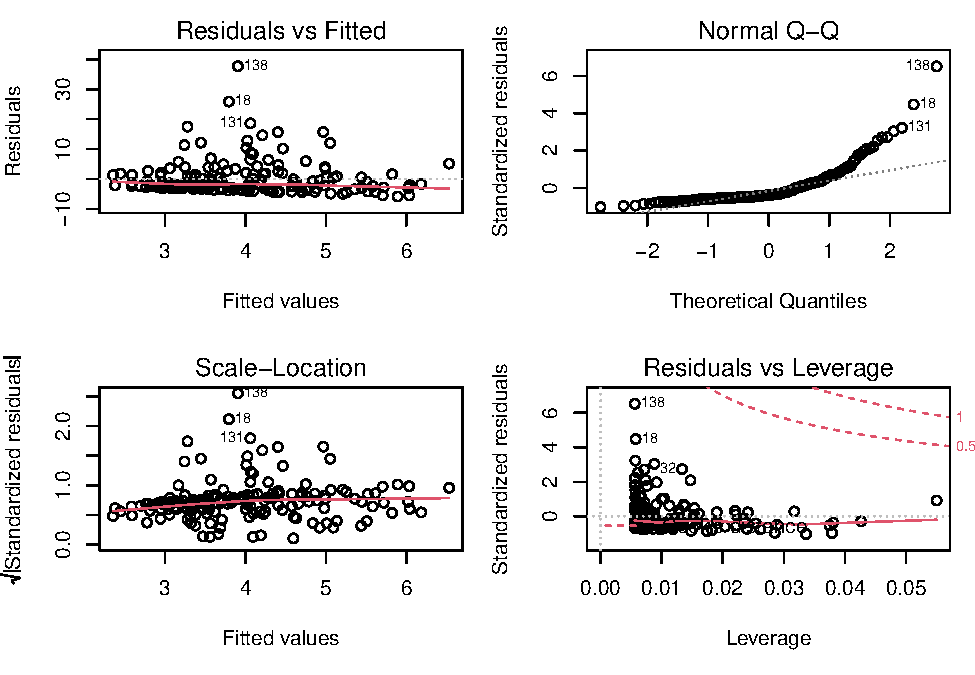
\includegraphics{Basic-Regression_files/figure-latex/unnamed-chunk-1-1.pdf}

Coefficient estimate: 0.0621

pvalue = 0.046

\hypertarget{deaths-per-capita-with-overall-ghsi-score}{%
\subsection{Deaths per capita with overall GHSI
score}\label{deaths-per-capita-with-overall-ghsi-score}}

\begin{Shaded}
\begin{Highlighting}[]
\FunctionTok{summary}\NormalTok{(}\FunctionTok{lm}\NormalTok{(deathpc }\SpecialCharTok{\textasciitilde{}}\NormalTok{ overall, }\AttributeTok{data =}\NormalTok{ sixmonth\_data))}\SpecialCharTok{$}\NormalTok{coef}
\end{Highlighting}
\end{Shaded}

\begin{verbatim}
##                 Estimate   Std. Error   t value     Pr(>|t|)
## (Intercept) -0.084278158 0.0415788685 -2.026947 4.416819e-02
## overall      0.004615341 0.0009437902  4.890219 2.250551e-06
\end{verbatim}

\begin{Shaded}
\begin{Highlighting}[]
\FunctionTok{par}\NormalTok{(}\AttributeTok{mfrow=}\FunctionTok{c}\NormalTok{(}\DecValTok{2}\NormalTok{,}\DecValTok{2}\NormalTok{),}\AttributeTok{mar=}\FunctionTok{c}\NormalTok{(}\DecValTok{5}\NormalTok{,}\DecValTok{4}\NormalTok{,}\DecValTok{2}\NormalTok{,}\DecValTok{1}\NormalTok{))}

\FunctionTok{plot}\NormalTok{(}\FunctionTok{lm}\NormalTok{(deathpc }\SpecialCharTok{\textasciitilde{}}\NormalTok{ overall, }\AttributeTok{data =}\NormalTok{ sixmonth\_data))}
\end{Highlighting}
\end{Shaded}

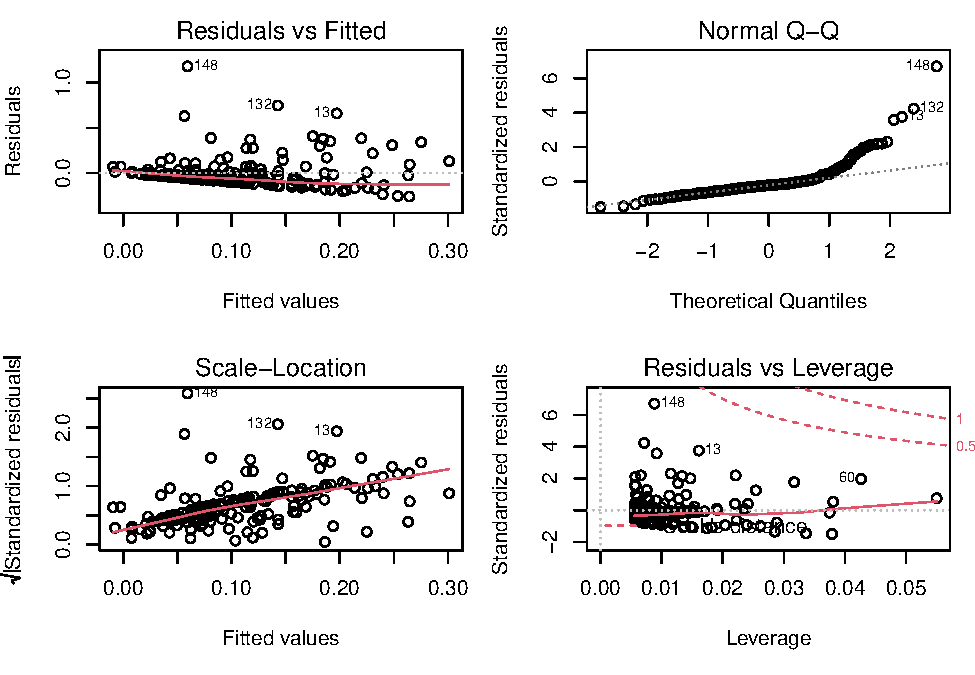
\includegraphics{Basic-Regression_files/figure-latex/unnamed-chunk-2-1.pdf}

Coefficient estimate: 0.0046

pvalue \textless{} .0001

\hypertarget{case-fatality-ratio-with-overall-ghsi-score}{%
\subsection{Case Fatality Ratio with overall GHSI
score}\label{case-fatality-ratio-with-overall-ghsi-score}}

\begin{Shaded}
\begin{Highlighting}[]
\FunctionTok{summary}\NormalTok{(}\FunctionTok{lm}\NormalTok{(cfratio }\SpecialCharTok{\textasciitilde{}}\NormalTok{ overall, }\AttributeTok{data =}\NormalTok{ sixmonth\_data))}\SpecialCharTok{$}\NormalTok{coef}
\end{Highlighting}
\end{Shaded}

\begin{verbatim}
##                Estimate Std. Error    t value     Pr(>|t|)
## (Intercept) -0.33252295 0.57139214 -0.5819523 5.613393e-01
## overall      0.07363439 0.01296991  5.6773234 5.509572e-08
\end{verbatim}

\begin{Shaded}
\begin{Highlighting}[]
\FunctionTok{par}\NormalTok{(}\AttributeTok{mfrow=}\FunctionTok{c}\NormalTok{(}\DecValTok{2}\NormalTok{,}\DecValTok{2}\NormalTok{),}\AttributeTok{mar=}\FunctionTok{c}\NormalTok{(}\DecValTok{5}\NormalTok{,}\DecValTok{4}\NormalTok{,}\DecValTok{2}\NormalTok{,}\DecValTok{1}\NormalTok{))}

\FunctionTok{plot}\NormalTok{(}\FunctionTok{lm}\NormalTok{(cfratio }\SpecialCharTok{\textasciitilde{}}\NormalTok{ overall, }\AttributeTok{data =}\NormalTok{ sixmonth\_data))}
\end{Highlighting}
\end{Shaded}

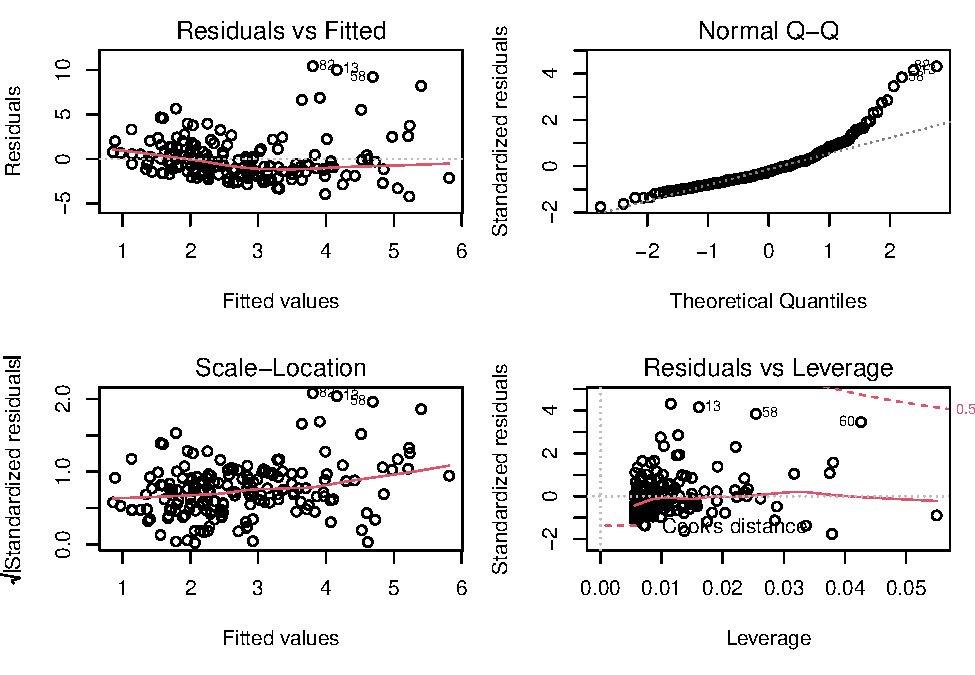
\includegraphics{Basic-Regression_files/figure-latex/unnamed-chunk-3-1.pdf}

Coefficient estimate: 0.074

pvalue \textless{} .0001

\hypertarget{question-2}{%
\subsection{Question 2}\label{question-2}}

\hypertarget{cases-per-capita-with-each-subcomponent}{%
\subsection{Cases per capita with each
subcomponent}\label{cases-per-capita-with-each-subcomponent}}

\begin{Shaded}
\begin{Highlighting}[]
\NormalTok{subcomponents }\OtherTok{\textless{}{-}} \FunctionTok{c}\NormalTok{(}\StringTok{"prev\_emergence\_pathogens"}\NormalTok{, }\StringTok{"early\_detection"}\NormalTok{, }\StringTok{"rapid\_response"}\NormalTok{, }\StringTok{"robust\_health\_sector"}\NormalTok{, }\StringTok{"commitments"}\NormalTok{, }\StringTok{"risk\_environment"}\NormalTok{)}

\ControlFlowTok{for}\NormalTok{(i }\ControlFlowTok{in} \DecValTok{1}\SpecialCharTok{:}\FunctionTok{length}\NormalTok{(subcomponents)) \{}
\NormalTok{  predictor\_i }\OtherTok{\textless{}{-}}\NormalTok{ (subcomponents)[i]}
  \FunctionTok{print}\NormalTok{(predictor\_i)}
  \FunctionTok{print}\NormalTok{(}\FunctionTok{summary}\NormalTok{(}\FunctionTok{lm}\NormalTok{(casepc }\SpecialCharTok{\textasciitilde{}}\NormalTok{ ., }\AttributeTok{data =}\NormalTok{ sixmonth\_data[,}\FunctionTok{c}\NormalTok{(}\StringTok{"casepc"}\NormalTok{,predictor\_i)]))}\SpecialCharTok{$}\NormalTok{coef)}
  \FunctionTok{par}\NormalTok{(}\AttributeTok{mfrow=}\FunctionTok{c}\NormalTok{(}\DecValTok{2}\NormalTok{,}\DecValTok{2}\NormalTok{),}\AttributeTok{mar=}\FunctionTok{c}\NormalTok{(}\DecValTok{5}\NormalTok{,}\DecValTok{4}\NormalTok{,}\DecValTok{2}\NormalTok{,}\DecValTok{1}\NormalTok{))}
  \FunctionTok{plot}\NormalTok{(}\FunctionTok{lm}\NormalTok{(casepc }\SpecialCharTok{\textasciitilde{}}\NormalTok{ ., }\AttributeTok{data =}\NormalTok{ sixmonth\_data[,}\FunctionTok{c}\NormalTok{(}\StringTok{"casepc"}\NormalTok{,predictor\_i)]))}
\NormalTok{\}}
\end{Highlighting}
\end{Shaded}

\begin{verbatim}
## [1] "prev_emergence_pathogens"
##                            Estimate Std. Error  t value   Pr(>|t|)
## (Intercept)              2.03616007 1.05282360 1.933999 0.05470819
## prev_emergence_pathogens 0.05222066 0.02632479 1.983706 0.04883468
\end{verbatim}

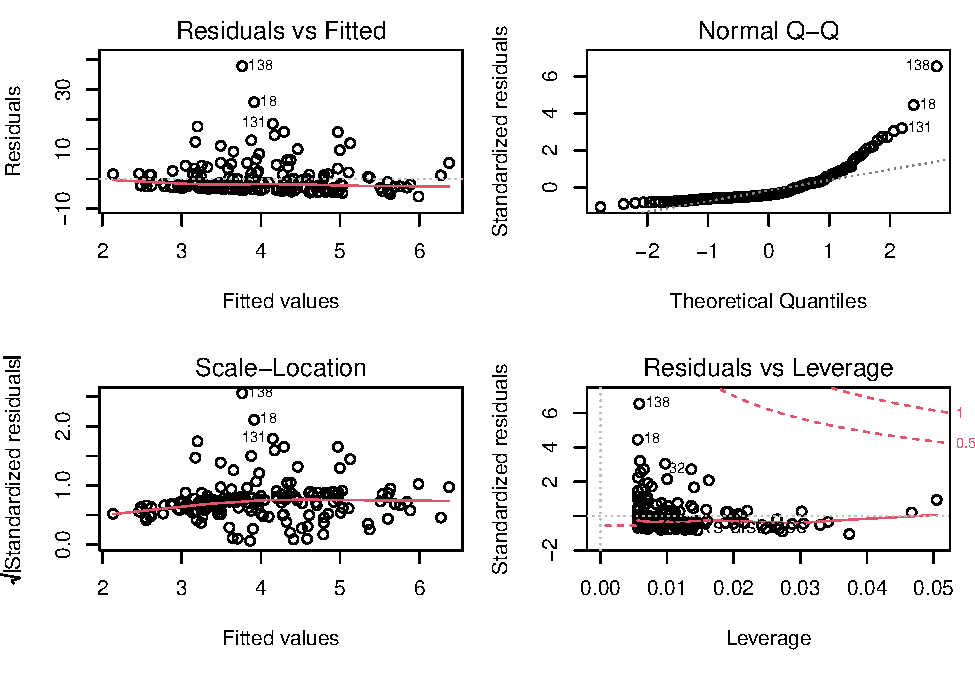
\includegraphics{Basic-Regression_files/figure-latex/unnamed-chunk-4-1.pdf}

\begin{verbatim}
## [1] "early_detection"
##                   Estimate Std. Error  t value    Pr(>|t|)
## (Intercept)     2.98123290 0.96009453 3.105145 0.002215175
## early_detection 0.02148599 0.01917076 1.120768 0.263904789
\end{verbatim}

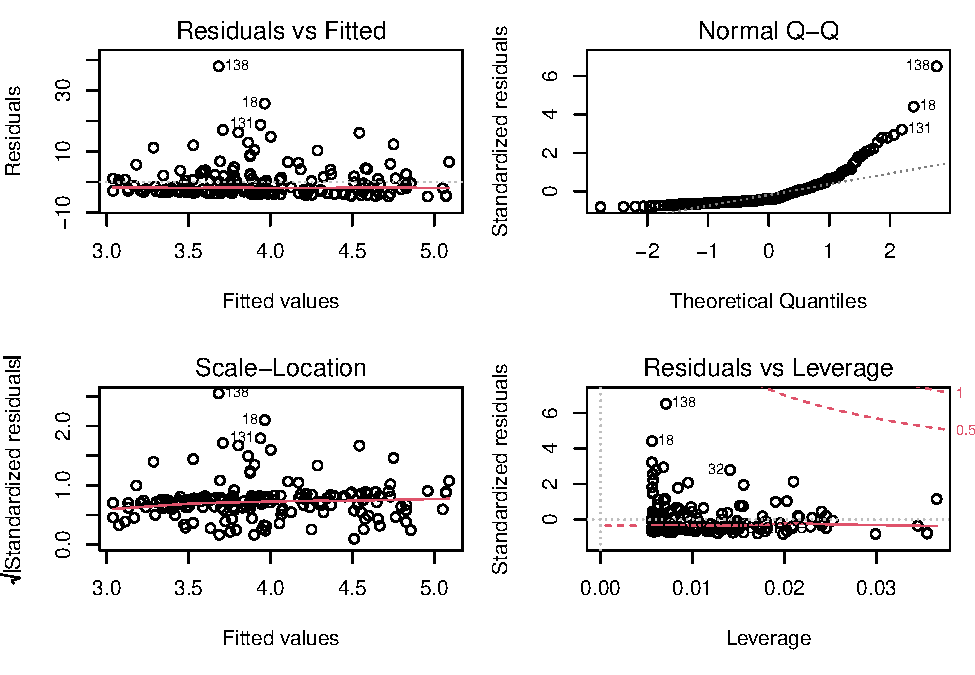
\includegraphics{Basic-Regression_files/figure-latex/unnamed-chunk-4-2.pdf}

\begin{verbatim}
## [1] "rapid_response"
##                 Estimate Std. Error  t value  Pr(>|t|)
## (Intercept)    1.3121490 1.24044803 1.057802 0.2915870
## rapid_response 0.0660832 0.02924656 2.259521 0.0250703
\end{verbatim}

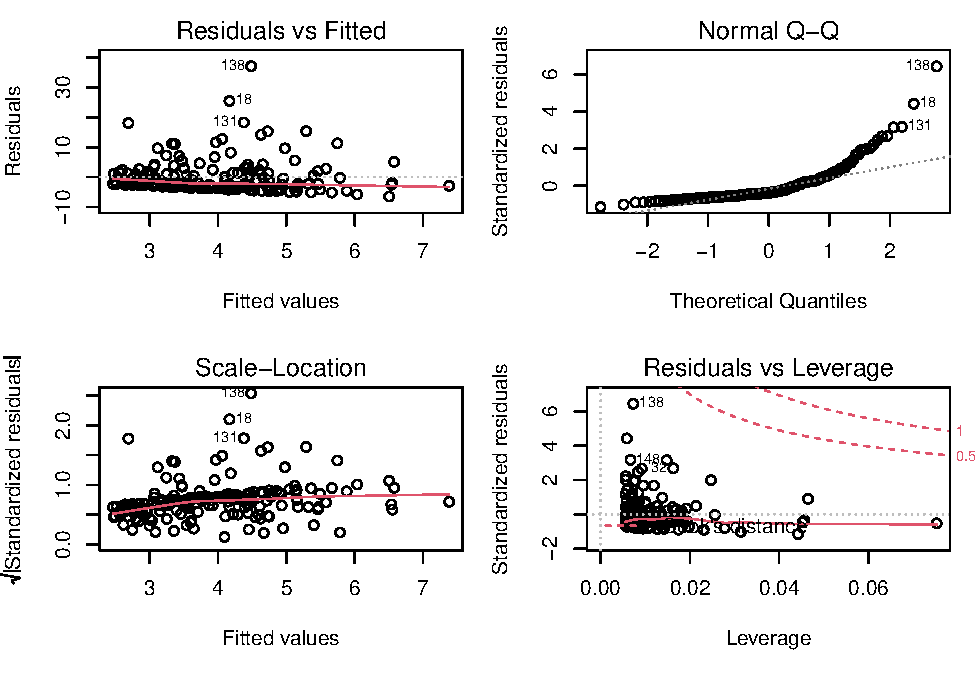
\includegraphics{Basic-Regression_files/figure-latex/unnamed-chunk-4-3.pdf}

\begin{verbatim}
## [1] "robust_health_sector"
##                        Estimate Std. Error  t value   Pr(>|t|)
## (Intercept)          2.13989642 0.83099480 2.575102 0.01083826
## robust_health_sector 0.06467009 0.02554554 2.531561 0.01222599
\end{verbatim}

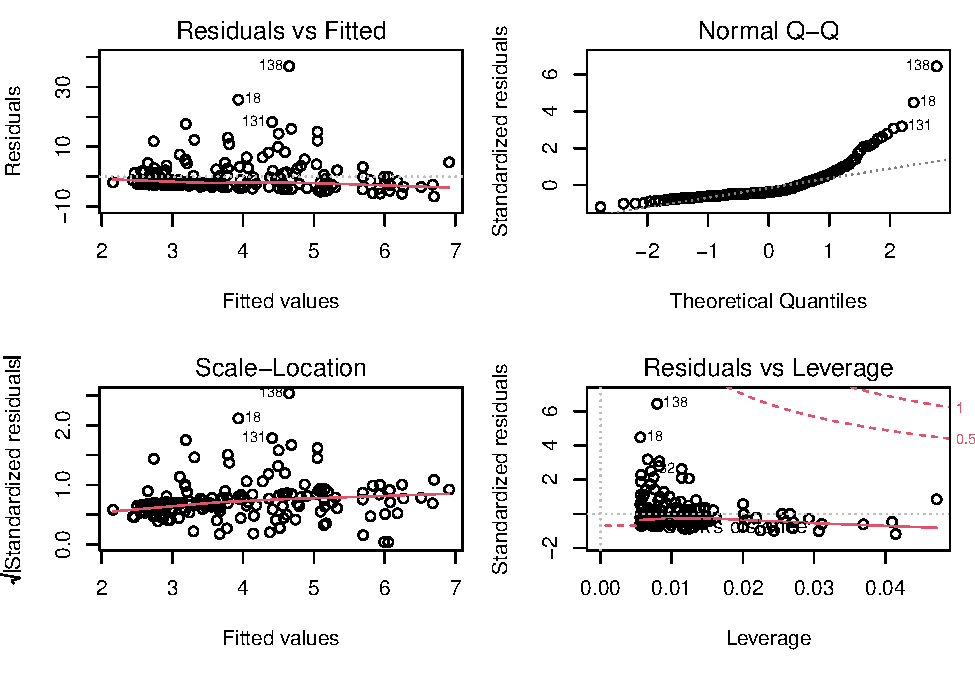
\includegraphics{Basic-Regression_files/figure-latex/unnamed-chunk-4-4.pdf}

\begin{verbatim}
## [1] "commitments"
##                Estimate Std. Error   t value     Pr(>|t|)
## (Intercept)  7.10083850 1.81375263  3.914998 0.0001288596
## commitments -0.06348428 0.03536646 -1.795042 0.0743531599
\end{verbatim}

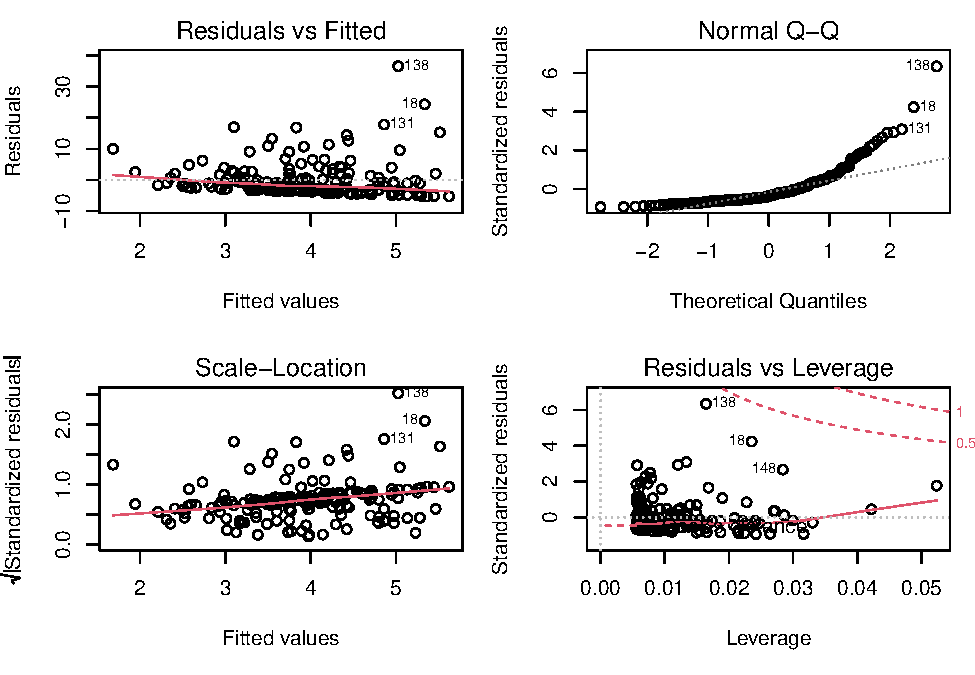
\includegraphics{Basic-Regression_files/figure-latex/unnamed-chunk-4-5.pdf}

\begin{verbatim}
## [1] "risk_environment"
##                    Estimate Std. Error   t value     Pr(>|t|)
## (Intercept)      -1.5801667 1.47958117 -1.067982 0.2869828581
## risk_environment  0.0993726 0.02553893  3.891025 0.0001411628
\end{verbatim}

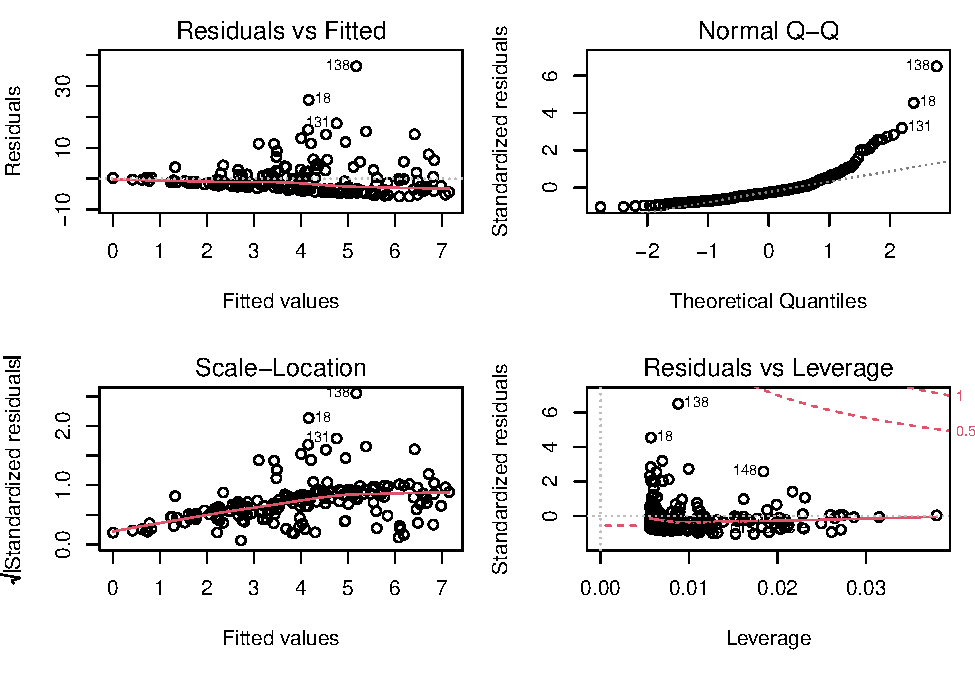
\includegraphics{Basic-Regression_files/figure-latex/unnamed-chunk-4-6.pdf}

\hypertarget{deaths-per-capita-with-each-subcomponent}{%
\subsection{Deaths per capita with each
subcomponent}\label{deaths-per-capita-with-each-subcomponent}}

\begin{Shaded}
\begin{Highlighting}[]
\NormalTok{subcomponents }\OtherTok{\textless{}{-}} \FunctionTok{c}\NormalTok{(}\StringTok{"prev\_emergence\_pathogens"}\NormalTok{, }\StringTok{"early\_detection"}\NormalTok{, }\StringTok{"rapid\_response"}\NormalTok{, }\StringTok{"robust\_health\_sector"}\NormalTok{, }\StringTok{"commitments"}\NormalTok{, }\StringTok{"risk\_environment"}\NormalTok{)}

\ControlFlowTok{for}\NormalTok{(i }\ControlFlowTok{in} \DecValTok{1}\SpecialCharTok{:}\FunctionTok{length}\NormalTok{(subcomponents)) \{}
\NormalTok{  predictor\_i }\OtherTok{\textless{}{-}}\NormalTok{ (subcomponents)[i]}
  \FunctionTok{print}\NormalTok{(predictor\_i)}
  \FunctionTok{print}\NormalTok{(}\FunctionTok{summary}\NormalTok{(}\FunctionTok{lm}\NormalTok{(deathpc }\SpecialCharTok{\textasciitilde{}}\NormalTok{ ., }\AttributeTok{data =}\NormalTok{ sixmonth\_data[,}\FunctionTok{c}\NormalTok{(}\StringTok{"deathpc"}\NormalTok{,predictor\_i)]))}\SpecialCharTok{$}\NormalTok{coef)}
  \FunctionTok{par}\NormalTok{(}\AttributeTok{mfrow=}\FunctionTok{c}\NormalTok{(}\DecValTok{2}\NormalTok{,}\DecValTok{2}\NormalTok{),}\AttributeTok{mar=}\FunctionTok{c}\NormalTok{(}\DecValTok{5}\NormalTok{,}\DecValTok{4}\NormalTok{,}\DecValTok{2}\NormalTok{,}\DecValTok{1}\NormalTok{))}
  \FunctionTok{plot}\NormalTok{(}\FunctionTok{lm}\NormalTok{(deathpc }\SpecialCharTok{\textasciitilde{}}\NormalTok{ ., }\AttributeTok{data =}\NormalTok{ sixmonth\_data[,}\FunctionTok{c}\NormalTok{(}\StringTok{"deathpc"}\NormalTok{,predictor\_i)]))}
\NormalTok{\}}
\end{Highlighting}
\end{Shaded}

\begin{verbatim}
## [1] "prev_emergence_pathogens"
##                              Estimate   Std. Error   t value     Pr(>|t|)
## (Intercept)              -0.033147977 0.0322456879 -1.027982 3.053612e-01
## prev_emergence_pathogens  0.003884845 0.0008062709  4.818287 3.099873e-06
\end{verbatim}

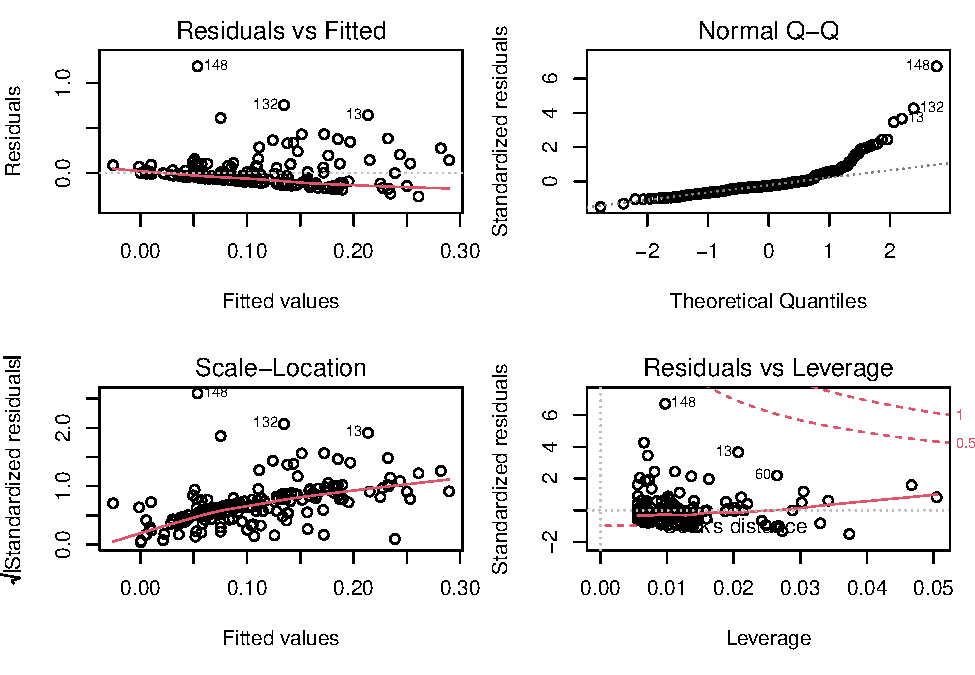
\includegraphics{Basic-Regression_files/figure-latex/unnamed-chunk-5-1.pdf}

\begin{verbatim}
## [1] "early_detection"
##                    Estimate   Std. Error   t value     Pr(>|t|)
## (Intercept)     0.005811494 0.0298091995 0.1949564 0.8456506927
## early_detection 0.002301133 0.0005952175 3.8660372 0.0001551698
\end{verbatim}

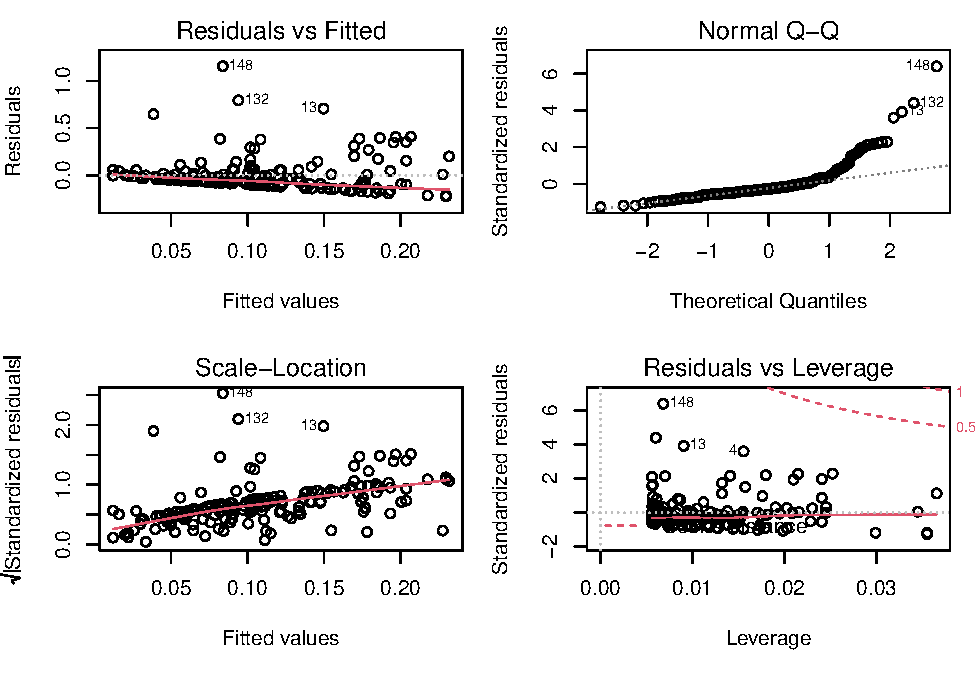
\includegraphics{Basic-Regression_files/figure-latex/unnamed-chunk-5-2.pdf}

\begin{verbatim}
## [1] "rapid_response"
##                    Estimate   Std. Error    t value     Pr(>|t|)
## (Intercept)    -0.031463871 0.0389541543 -0.8077154 0.4203385866
## rapid_response  0.003519134 0.0009184382  3.8316499 0.0001766153
\end{verbatim}

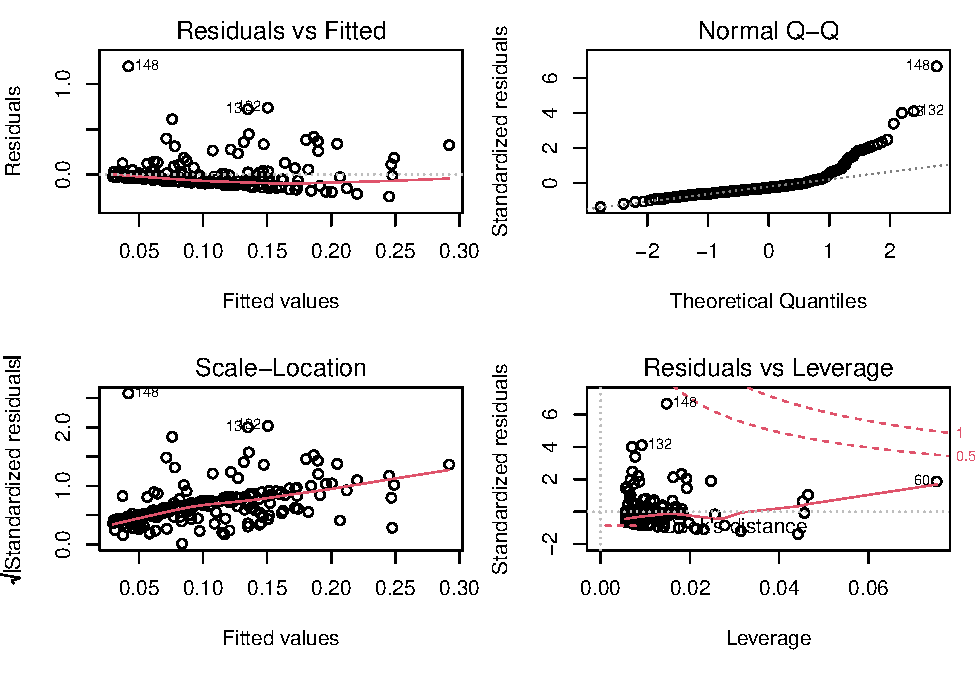
\includegraphics{Basic-Regression_files/figure-latex/unnamed-chunk-5-3.pdf}

\begin{verbatim}
## [1] "robust_health_sector"
##                         Estimate   Std. Error   t value     Pr(>|t|)
## (Intercept)          0.005398486 0.0257055625 0.2100124 8.338996e-01
## robust_health_sector 0.003703231 0.0007902124 4.6863743 5.528390e-06
\end{verbatim}

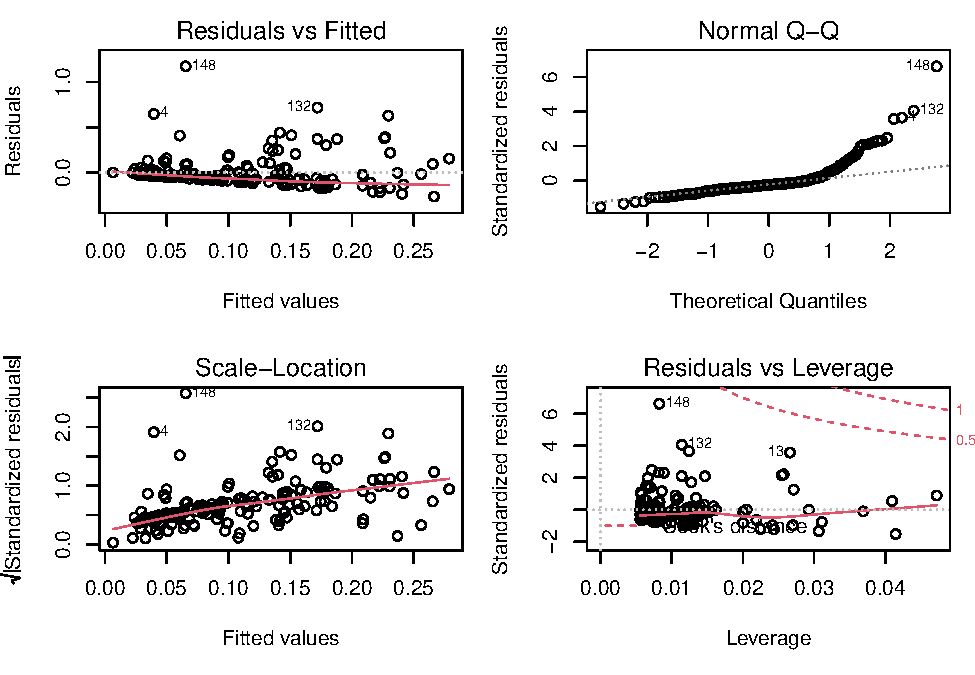
\includegraphics{Basic-Regression_files/figure-latex/unnamed-chunk-5-4.pdf}

\begin{verbatim}
## [1] "commitments"
##                Estimate Std. Error   t value  Pr(>|t|)
## (Intercept) 0.016526439 0.05853463 0.2823361 0.7780157
## commitments 0.001846263 0.00114137 1.6175856 0.1075326
\end{verbatim}

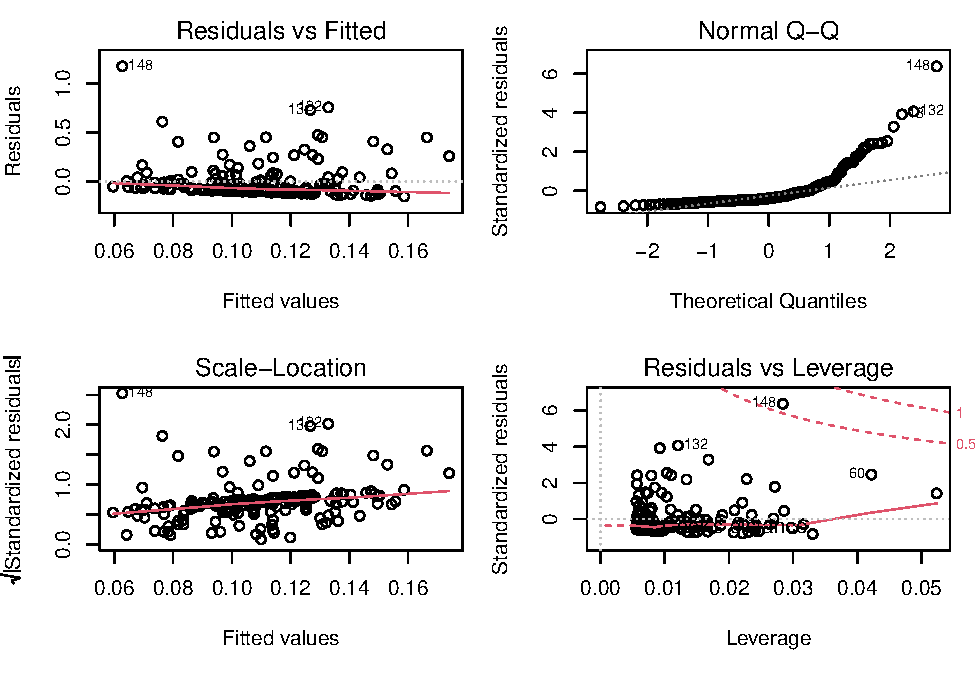
\includegraphics{Basic-Regression_files/figure-latex/unnamed-chunk-5-5.pdf}

\begin{verbatim}
## [1] "risk_environment"
##                     Estimate   Std. Error   t value     Pr(>|t|)
## (Intercept)      -0.11767540 0.0463950265 -2.536380 1.206497e-02
## risk_environment  0.00407107 0.0008008207  5.083623 9.362623e-07
\end{verbatim}

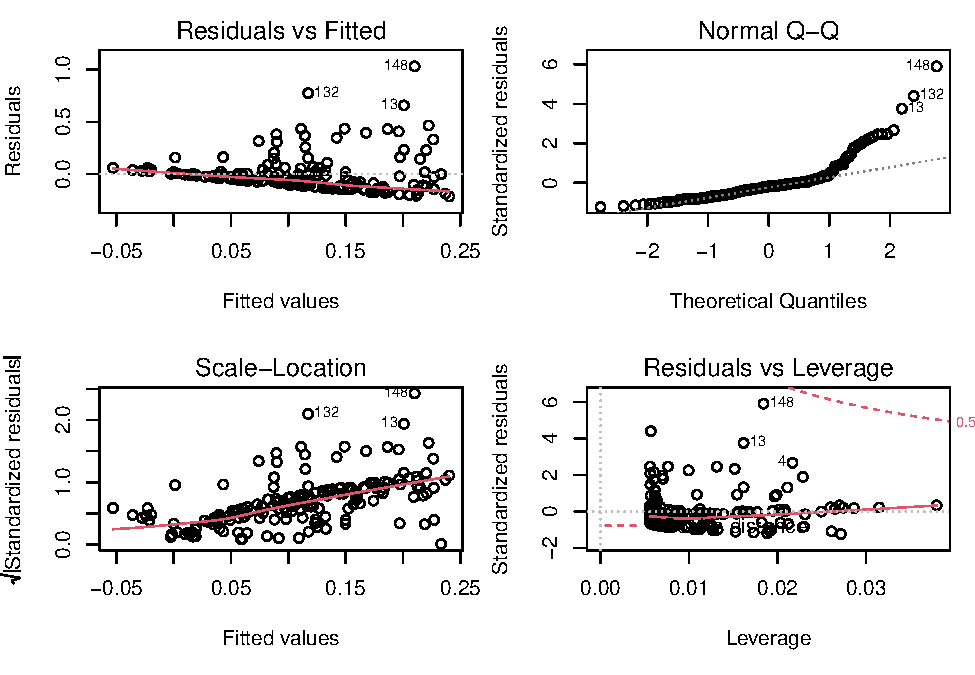
\includegraphics{Basic-Regression_files/figure-latex/unnamed-chunk-5-6.pdf}

\hypertarget{case-fatality-ratio-with-each-subcomponent}{%
\subsection{Case Fatality Ratio with each
subcomponent}\label{case-fatality-ratio-with-each-subcomponent}}

\begin{Shaded}
\begin{Highlighting}[]
\NormalTok{subcomponents }\OtherTok{\textless{}{-}} \FunctionTok{c}\NormalTok{(}\StringTok{"prev\_emergence\_pathogens"}\NormalTok{, }\StringTok{"early\_detection"}\NormalTok{, }\StringTok{"rapid\_response"}\NormalTok{, }\StringTok{"robust\_health\_sector"}\NormalTok{, }\StringTok{"commitments"}\NormalTok{, }\StringTok{"risk\_environment"}\NormalTok{)}

\ControlFlowTok{for}\NormalTok{(i }\ControlFlowTok{in} \DecValTok{1}\SpecialCharTok{:}\FunctionTok{length}\NormalTok{(subcomponents)) \{}
\NormalTok{  predictor\_i }\OtherTok{\textless{}{-}}\NormalTok{ (subcomponents)[i]}
  \FunctionTok{print}\NormalTok{(predictor\_i)}
  \FunctionTok{print}\NormalTok{(}\FunctionTok{summary}\NormalTok{(}\FunctionTok{lm}\NormalTok{(cfratio }\SpecialCharTok{\textasciitilde{}}\NormalTok{ ., }\AttributeTok{data =}\NormalTok{ sixmonth\_data[,}\FunctionTok{c}\NormalTok{(}\StringTok{"cfratio"}\NormalTok{,predictor\_i)]))}\SpecialCharTok{$}\NormalTok{coef)}
  \FunctionTok{par}\NormalTok{(}\AttributeTok{mfrow=}\FunctionTok{c}\NormalTok{(}\DecValTok{2}\NormalTok{,}\DecValTok{2}\NormalTok{),}\AttributeTok{mar=}\FunctionTok{c}\NormalTok{(}\DecValTok{5}\NormalTok{,}\DecValTok{4}\NormalTok{,}\DecValTok{2}\NormalTok{,}\DecValTok{1}\NormalTok{))}
  \FunctionTok{plot}\NormalTok{(}\FunctionTok{lm}\NormalTok{(cfratio }\SpecialCharTok{\textasciitilde{}}\NormalTok{ ., }\AttributeTok{data =}\NormalTok{ sixmonth\_data[,}\FunctionTok{c}\NormalTok{(}\StringTok{"cfratio"}\NormalTok{,predictor\_i)]))}
\NormalTok{\}}
\end{Highlighting}
\end{Shaded}

\begin{verbatim}
## [1] "prev_emergence_pathogens"
##                            Estimate Std. Error   t value     Pr(>|t|)
## (Intercept)              0.41630850 0.44104052 0.9439235 3.464954e-01
## prev_emergence_pathogens 0.06381554 0.01102777 5.7868016 3.196661e-08
\end{verbatim}

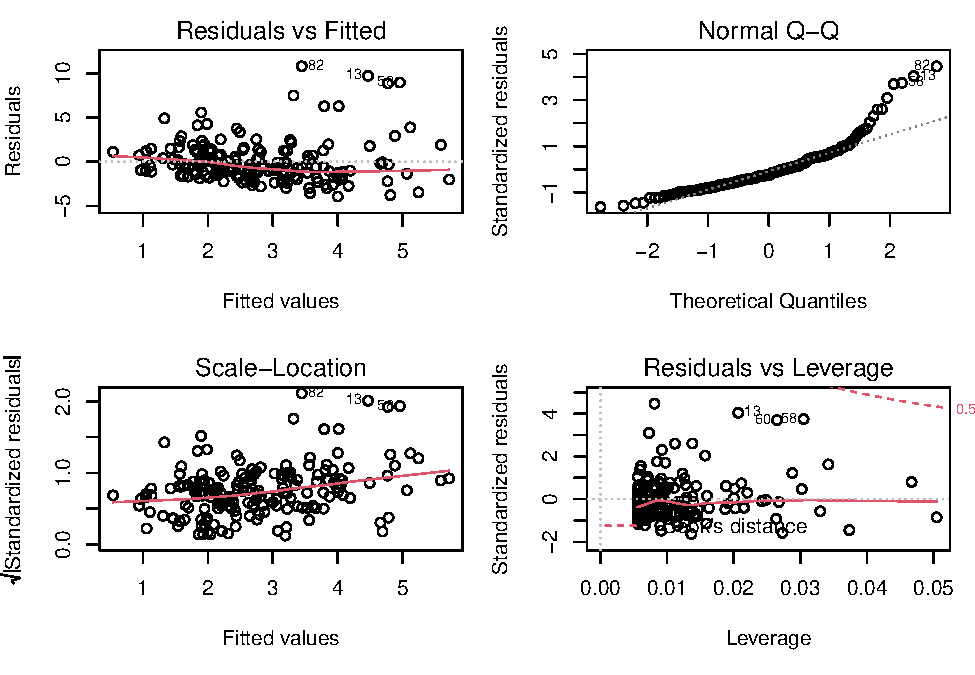
\includegraphics{Basic-Regression_files/figure-latex/unnamed-chunk-6-1.pdf}

\begin{verbatim}
## [1] "early_detection"
##                  Estimate  Std. Error  t value     Pr(>|t|)
## (Intercept)     1.0189258 0.410319789 2.483248 1.394981e-02
## early_detection 0.0386378 0.008193093 4.715900 4.861683e-06
\end{verbatim}

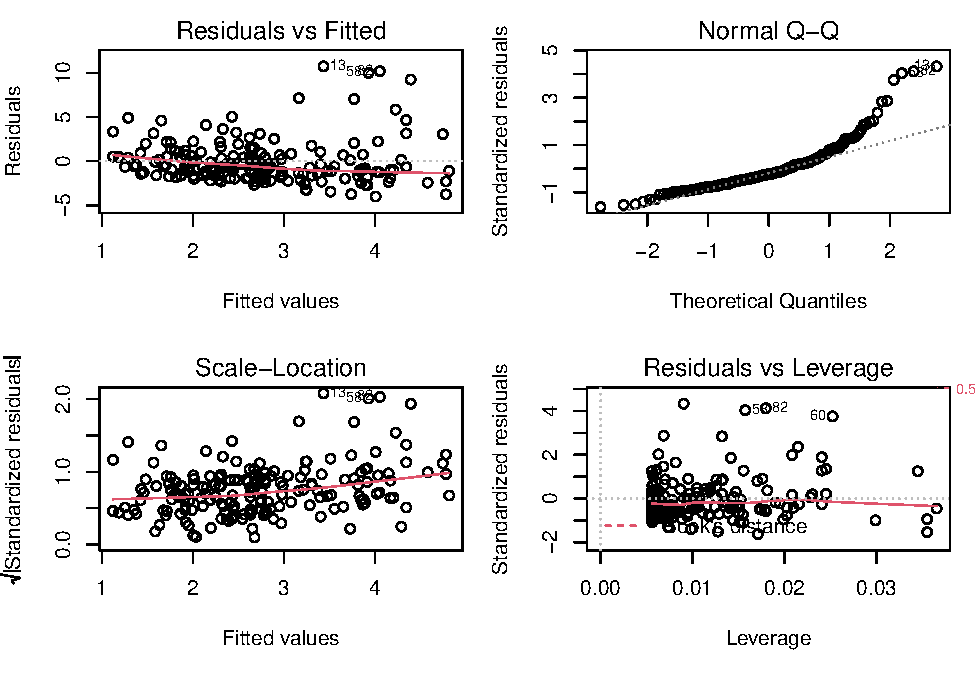
\includegraphics{Basic-Regression_files/figure-latex/unnamed-chunk-6-2.pdf}

\begin{verbatim}
## [1] "rapid_response"
##                  Estimate Std. Error   t value     Pr(>|t|)
## (Intercept)    0.45649178 0.53813891 0.8482787 3.974285e-01
## rapid_response 0.05749323 0.01268792 4.5313348 1.075448e-05
\end{verbatim}

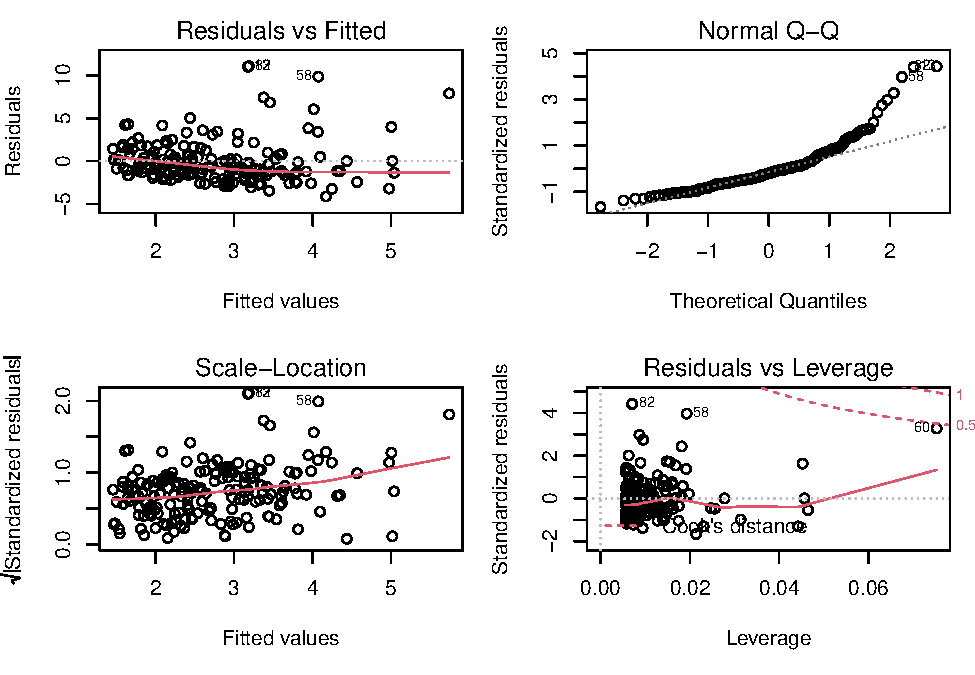
\includegraphics{Basic-Regression_files/figure-latex/unnamed-chunk-6-3.pdf}

\begin{verbatim}
## [1] "robust_health_sector"
##                        Estimate Std. Error  t value     Pr(>|t|)
## (Intercept)          1.11897822 0.35459144 3.155683 1.882132e-03
## robust_health_sector 0.05833582 0.01090046 5.351683 2.673197e-07
\end{verbatim}

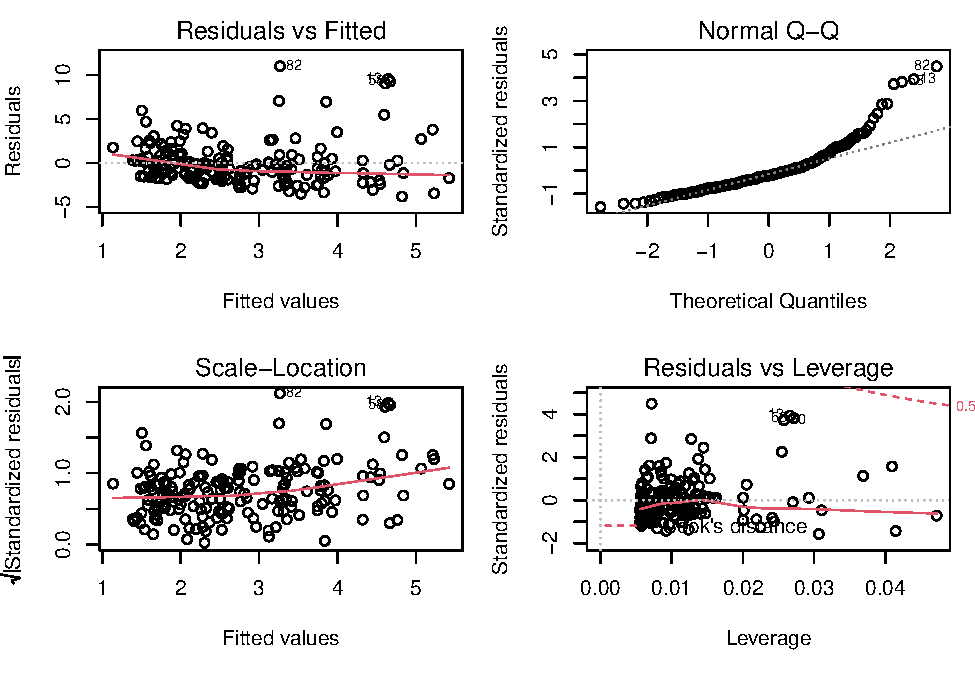
\includegraphics{Basic-Regression_files/figure-latex/unnamed-chunk-6-4.pdf}

\begin{verbatim}
## [1] "commitments"
##                Estimate Std. Error    t value    Pr(>|t|)
## (Intercept) -0.26959584 0.79337580 -0.3398085 0.734403638
## commitments  0.06049012 0.01547008  3.9101371 0.000131269
\end{verbatim}

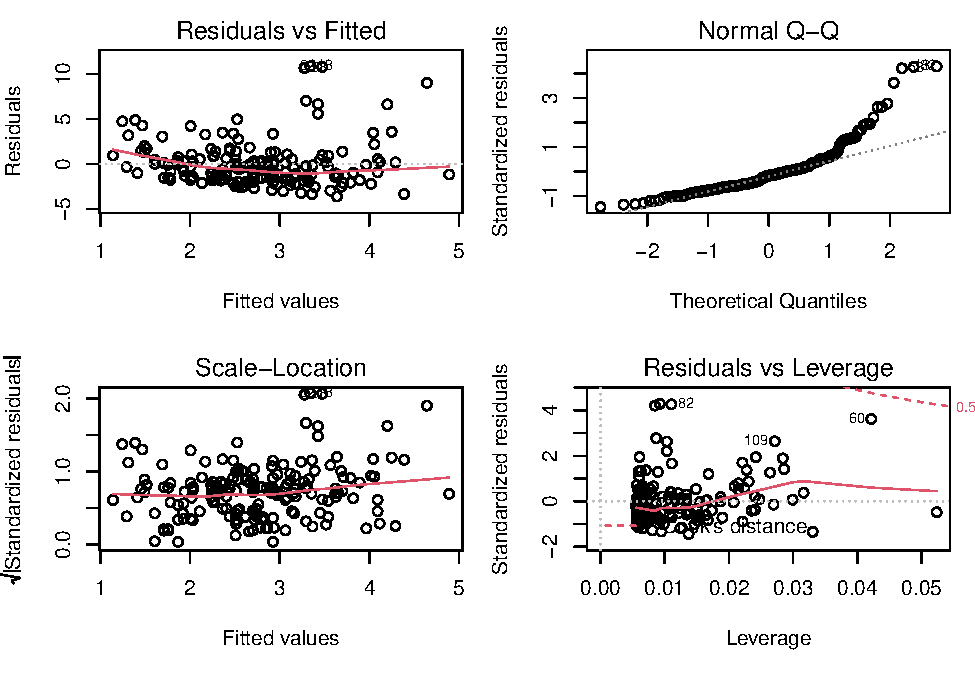
\includegraphics{Basic-Regression_files/figure-latex/unnamed-chunk-6-5.pdf}

\begin{verbatim}
## [1] "risk_environment"
##                    Estimate Std. Error  t value    Pr(>|t|)
## (Intercept)      0.76031876 0.67896796 1.119815 0.264309685
## risk_environment 0.03568434 0.01171961 3.044840 0.002683559
\end{verbatim}

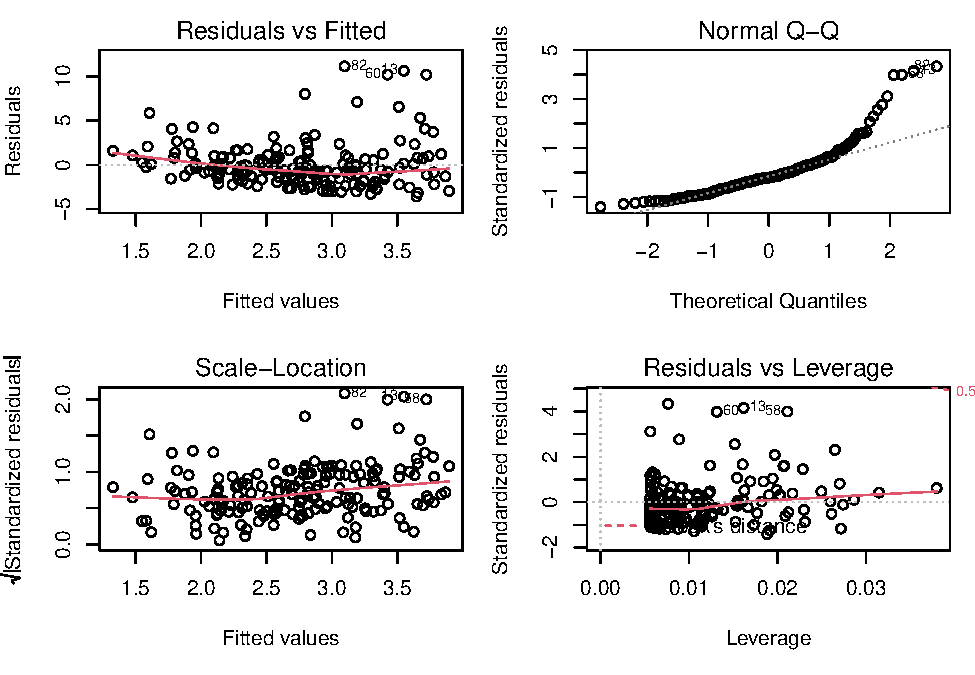
\includegraphics{Basic-Regression_files/figure-latex/unnamed-chunk-6-6.pdf}

\end{document}
